\documentclass{beamer}
\usepackage{graphicx}
\usepackage{amsmath}
\usepackage{amssymb}
\usepackage{booktabs}
\usepackage{pgfplots}
\usepackage{tikz}
\usetikzlibrary{shapes.geometric, arrows}
\usetikzlibrary{positioning}
\usepackage{background}
\pgfplotsset{width=0.5\textwidth, compat=1.11}
\definecolor{myblue}{RGB}{0, 102, 204}
\setbeamercolor{frametitle}{fg=white,bg=myblue}
% Set the background image
    \backgroundsetup{
    scale=0.6,
    color=black,
    opacity=0.5, % Adjust opacity of the background image
    contents={\includegraphics[width=\paperwidth,height=\paperheight]{bg.jpg}}
}


\tikzstyle{startstop} = [rectangle, rounded corners, minimum width=1cm, minimum height=0.2cm, text centered, draw=black, fill=red!30]
\tikzstyle{process} = [rectangle, minimum width=1cm, minimum height=1cm, text centered, draw=black, fill=orange!30]
\tikzstyle{decision} = [diamond, minimum width=1cm, minimum height=1cm, text centered, draw=black, fill=yellow!30]
\tikzstyle{arrow} = [thick,->,>=stealth]

\title{The Detection and Prevention of Cloud Computing Attacks Using Artificial Intelligence Technologies}
\author{Razib Dash}
\date{March 13, 2025}
\institute{
  Batch: 56th (B)\\
  ID: 221-115-075\\
  Department of computer science and engineering\\
  Metropolitan University
}
\begin{document}

\begin{frame}
\begin{center}
  
   
\end{center}
  \titlepage
\end{frame}

\begin{frame}{Introduction}
\begin{itemize}
    \item Cloud computing has revolutionized data management and storage.
    \item Increased reliance on cloud services has led to a rise in cyber-attacks.
    \item Traditional security measures are insufficient against evolving threats.
    \item Artificial Intelligence (AI) offers promising solutions for cloud security.
\end{itemize}
\end{frame}

\begin{frame}{Motivation and Objectives}
\framesubtitle{Motivation}
\begin{itemize}
    \item Rapid adoption of cloud computing services.
    \item Security challenges: data breaches, unauthorized access, malicious activities.
    \item Ensuring integrity, confidentiality, and availability of sensitive information.
\end{itemize}

\framesubtitle{Objectives}
\begin{itemize}
    \item Investigate the current landscape of cloud computing security.
    \item Explore the application of AI for detecting and preventing attacks.
    \item Provide insights and recommendations for effective implementation.
\end{itemize}
\end{frame}

\begin{frame}{Cloud Computing Overview}
\begin{itemize}
    \item Cloud computing delivers computing services over the internet.
    \item Models: Infrastructure as a Service (IaaS), Platform as a Service (PaaS), Software as a Service (SaaS).
    \item Benefits: Scalability, cost-effectiveness, global collaboration.
\end{itemize}

\begin{figure}[h]
    \centering
    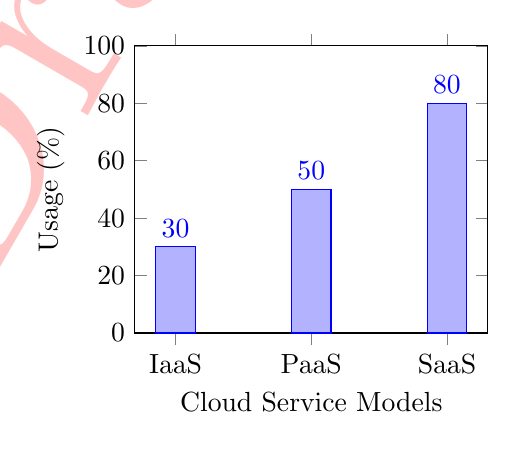
\begin{tikzpicture}
        \begin{axis}[
            ybar,
            ymin=0,
            ymax=100,
            xlabel={Cloud Service Models},
            ylabel={Usage (\%)},
            symbolic x coords={IaaS, PaaS, SaaS},
            xtick=data,
            nodes near coords,
            bar width=0.5cm,
            enlarge x limits=0.15,
            legend style={at={(0.5,-0.2)}, anchor=north, legend columns=-1},
        ]
            \addplot coordinates {(IaaS, 30) (PaaS, 50) (SaaS, 80)};
            % \legend{Usage};
        \end{axis}
    \end{tikzpicture}
    \caption{Cloud Pyramid: Usage of IaaS, PaaS, and SaaS}
    \label{fig:cloud_pyramid}
\end{figure}
\end{frame}

\begin{frame}{Security Challenges in Cloud Computing}
\begin{itemize}
    \item Data breaches: Unauthorized access to sensitive information.
    \item Denial-of-Service (DoS) attacks: Overwhelming cloud servers with traffic.
    \item Insider threats: Malicious or negligent insiders compromising data.
\end{itemize}

\begin{figure}[h]
    \centering
    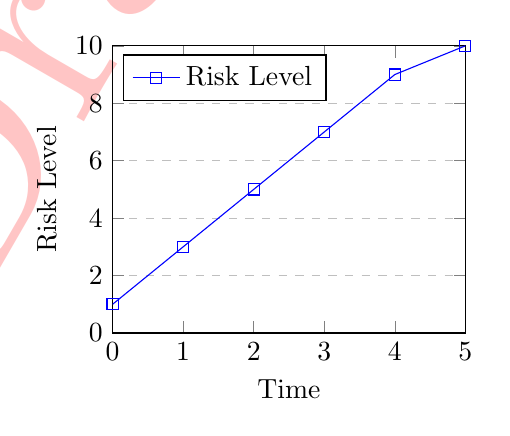
\begin{tikzpicture}
        \begin{axis}[
            xlabel={Time},
            ylabel={Risk Level},
            ymin=0, ymax=10,
            xmin=0, xmax=5,
            xtick={0,1,2,3,4,5},
            ytick={0,2,4,6,8,10},
            legend pos=north west,
            ymajorgrids=true,
            grid style=dashed,
        ]
            \addplot[
                color=blue,
                mark=square,
            ]
            coordinates {
                (0,1)(1,3)(2,5)(3,7)(4,9)(5,10)
            };
            \legend{Risk Level}
        \end{axis}
    \end{tikzpicture}
    \caption{Cloud Security Risks Over Time}
    \label{fig:cloud_security_risks}
\end{figure}
\end{frame}

\begin{frame}{AI Technologies for Cloud Security}
\framesubtitle{Machine Learning for Anomaly Detection}
\begin{figure}[h]
    \centering
    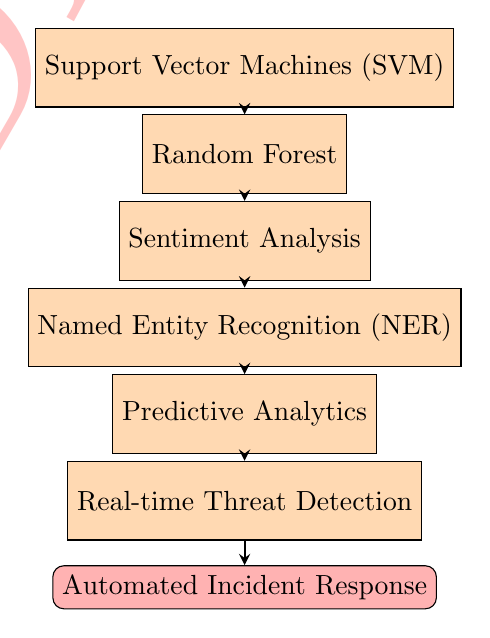
\begin{tikzpicture}[node distance=1.1cm]

        % Nodes
        \node (svm) [process] {Support Vector Machines (SVM)};
        \node (forest) [process, below of=svm] {Random Forest};
        \node (sentiment) [process, below of=forest] {Sentiment Analysis};
        \node (ner) [process, below of=sentiment] {Named Entity Recognition (NER)};
        \node (predictive) [process, below of=ner] {Predictive Analytics};
        \node (realtime) [process, below of=predictive] {Real-time Threat Detection};
        \node (response) [startstop, below of=realtime] {Automated Incident Response};

        % Arrows
        \draw [arrow] (svm) -- (forest);
        \draw [arrow] (forest) -- (sentiment);
        \draw [arrow] (sentiment) -- (ner);
        \draw [arrow] (ner) -- (predictive);
        \draw [arrow] (predictive) -- (realtime);
        \draw [arrow] (realtime) -- (response);

    \end{tikzpicture}
    \caption{Automated Incident Response Workflow}
    \label{fig:automated_response}
\end{figure}


\end{frame}

\begin{frame}
 \begin{itemize}
    \item Support Vector Machines (SVM): Classify and detect patterns.
    \item Random Forest: Ensemble learning for improved accuracy.
\end{itemize}

\framesubtitle{Natural Language Processing (NLP)}
\begin{itemize}
    \item Sentiment Analysis: Assess communication sentiment.
    \item Named Entity Recognition (NER): Identify and categorize entities.
\end{itemize}

\framesubtitle{Predictive Analytics}
\begin{itemize}
    \item Leverage historical data to predict security risks.
    \item Time series analysis for forecasting threats.
\end{itemize}

\framesubtitle{Automated Incident Response}
\begin{itemize}
    \item Real-time threat detection and mitigation.
    \item Intelligent automation for incident response.
\end{itemize}
\end{frame}
    

\begin{frame}{Recommendations}
\begin{itemize}
    \item Integrate AI technologies into cloud security frameworks.
    \item Implement continuous monitoring and analysis.
    \item Foster collaborative threat intelligence sharing.
    \item Conduct regular training and cybersecurity awareness programs.
\end{itemize}
\end{frame}

\begin{frame}{Conclusion}
\begin{itemize}
    \item Cloud computing offers opportunities but also presents security challenges.
    \item AI technologies provide proactive and adaptive solutions.
    \item Machine learning, NLP, predictive analytics, and automated incident response are key tools.
    \item Recommendations aim to fortify cloud security and adapt to the dynamic threat landscape.
\end{itemize}
    \begin{center}
    \Huge \textbf{Thank You!} \\[20pt]
        
    \end{center}
   

\end{frame}


\end{document}